% 导言区,进行全局设置
\documentclass[12pt]{ctexart}%book, report, latter, 引入文档类

%\usepackage{ctex}
%\usepackage[fleqn]{amsmath}
\usepackage{amsmath}
\usepackage{amssymb}
\usepackage{fancyhdr}
\usepackage{lastpage}
\usepackage{graphicx}
\usepackage{float}
\usepackage{enumerate} % when need define format to number by myself
\usepackage[colorlinks,linkcolor=black]{hyperref} % set super link
\usepackage{color} % set text color
\usepackage{subfigure} % set two picture on one line

\usepackage{geometry}
\geometry{a4paper,top=2.54cm,left=3.18cm,bottom=2.54cm,right=3.18cm,includehead,includefoot}

% \newcommand命令的定义,新的命令
\newcommand\degree{^\circ}
\title{\kaishu Deep Residual Learning for Image Recognition}
\author{Fish}
\date{\today}

\graphicspath{{figures/}} %图片在当前目录下的figures目录

% 内容与格式分离
% 设置标题的格式
\ctexset {
	section = {
		format+=\zihao {-4} \heiti \raggedright,
		%name = {,},
		%number = \chinese{section},
		beforeskip = 1.0ex plus 0.2ex minus .2ex,
		afterskip = 1.0ex plus 0.2ex minus .2ex,
		aftername = \hspace{0pt}
	},
	subsection = {
		format+=\zihao{5} \heiti \raggedright,
		% name={\thesubsection},
		name = {,},
		%number = \arabic{subsection},
		beforeskip = 1.0ex plus 0.2ex minus .2ex,
		afterskip = 1.0ex plus 0.2ex minus .2ex,
		aftername = \hspace{0pt}
	}
}


% 正文区(文稿区),有且只有一个document环境
% \begim{*环境名称}
%        内容
% \end{*环境名称}
\begin{document}
	\maketitle
	%\clearpage
	\renewcommand{\contentsname}{Content} % set the 目录 to Content
	\tableofcontents
	\clearpage
	\pagestyle{fancy}
	\lhead{Deep Residual Learning for Image Recognition}                   
	\rhead{Page \thepage{} of \pageref{LastPage}}
	\setcounter{page}{1}
	
	\section{\quad introduction}
		\subsection{\quad depth of network why it's so important?} 
			
			因为 CNN 能够提取 low/mid/high-level 的特征, 网络的层数越多, 意味着能够提取到不同 level 的特征越丰富, 并且, 越深的网络提取的特征越抽象, 越具有语义信息
			
		\subsection{\quad why not able to increase easily the number of network layer?} 
			\begin{enumerate}
				\item 对于原来的网络, 如果简单地增加深度, 会导致梯度弥散或梯度爆炸
				
				\item 对于该问题的解决方法时正则化初始化和中间的正则化层 (batch normalization), 这样可以训练几十层的网络
				
				\item 虽然此时通过 batch normalization 可以训练了,但出现另一个问题 \textcolor{red}{退化} 问题
					$\Rightarrow$
					网络层数增加, 但是在训练集上的准确率却饱和甚至下降了, 这个不能解释为 overfitting, 因为 过拟合 应该表现为在 训练集 上表现更好
			\end{enumerate}
		
		\subsection{\quad example} 
			\begin{figure}[H]
				\vspace{-0.2cm}  %调整图片与上文的垂直距离
				\setlength{\abovecaptionskip}{-0.2cm}   %调整图片标题与图距离
				%\setlength{\belowcaptionskip}{-1cm}   %调整图片标题与下文距离
				\centering
				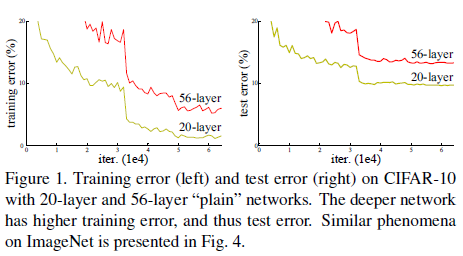
\includegraphics[scale=1]{degradation_problem.png}
				\renewcommand{\figurename}{Fig} % set picture title starting with Fig or 图
				\caption{degradation problem}
				\label{fig1:example}
			\end{figure}
		
		\subsection{\quad experiment and conclusion} 
			通过浅层网络 $y=x$ 等同映射构造深层模型,结果深层模型并没有比浅层网络有等同或更低的错误率,推断退化问题可能是因为深层的网络并不是那么好训练,也就是求解器很难去利用多层网络拟合同等函数。
			
			直白的说, \textcolor{red}{为什么层数多了准确率反而下降?}
			
			一个是56层的网络一个是20层的网络,从原理上来说其实56层网络的解空间是包括了20层网络的解空间的,换而言之也就是说,56层网络取得的性能应该大于等于20层网络的性能的。但是从训练的迭代过程来看,56层的网络无论从训练误差来看还是测试误差来看,误差都大于20层的网络(这也说明了为什么这不是过拟合现象,因为56层网络本身的训练误差都没有降下去)。\textcolor{red}{导致这个原因就是虽然56层网络的解空间包含了20层网络的解空间,但是我们在训练网络用的是随机梯度下降策略,往往解到的不是全局最优解,而是局部的最优解,显而易见56层网络的解空间更加的复杂,所以导致使用随机梯度下降算法无法解到最优解。}

	\section{\quad how to solve degradation problem}
		\subsection{\quad analysis}
			\begin{itemize}
				\item 上述退化问题的一个解决办法是\textcolor{red}{恒等映射}, 一个深层网络,如果后面的一大堆层都是恒等映射,那么这个深度网络其实就退化成了一个\textcolor{red}{浅层网络}
				
				\item 现在希望找到一个恒等映射函数 $H(x) = x$ 但是直接拟合出这个函数是有困难的, 不然深层网络也不会出现退化现象了. 于是我们把网络设计成一个残差函数
					\begin{align}
						F(x) = H(x) - x
					\end{align}
					
				\item 我们通过学习 $F(x)$, 并且令其等于 0, 就可以构成了一个恒等映射 $H(x) = x$, $F(x)$ 就是残差函数, 这就是残差的操作. 
			\end{itemize}

		\subsection{\quad theory}
			\begin{itemize}
				\item for degradation problem
				
					\qquad Resnet提供了两种选择方式,也就是identity mapping和residual mapping,如果网络已经到达最优,继续加深网络,residual mapping将被push为0,只剩下identity mapping,这样理论上网络一直处于最优状态了,网络的性能也就不会随着深度增加而降低了。

				\item combine instance to comprehend
					
					\qquad F是求和前网络映射,H是从输入到求和后的网络映射。比如把5映射到5.1,那么引入残差前是$F'(5)=5.1$,引入残差后是$H(5)=5.1, H(5)=F(5)+5, F(5)=0.1$。这里的F’和F都表示网络参数映射,引入残差后的映射对输出的变化更敏感。比如s输出从5.1变到5.2,映射$F'$的输出增加了$1/51=2\%$,而对于残差结构输出从5.1到5.2,映射F是从0.1到0.2,增加了$100\%$。明显后者输出变化对权重的调整作用更大,所以效果更好。残差的思想都是去掉相同的主体部分,从而突出微小的变化,看到残差网络我第一反应就是差分放大器…

				\item thinking more
				
					\qquad 残差的思想其实还是很像我们高数中学的泰勒公式的,在泰勒公式中,我们往后相加的是更高阶的多项式,这里加的也可以考虑成更高阶的多项式
			\end{itemize}		
		
	\section{\quad network architecture and formula derivation}
			\subsection{\quad network architecture}
						\begin{figure}[H]
							\vspace{-0.2cm}  %调整图片与上文的垂直距离
							\setlength{\abovecaptionskip}{-0.2cm}   %调整图片标题与图距离
							%\setlength{\belowcaptionskip}{-1cm}   %调整图片标题与下文距离
							\centering
							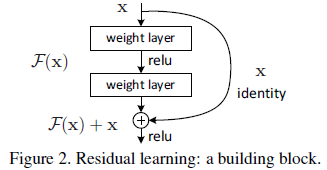
\includegraphics[scale=1]{network_architecture.png}
							\renewcommand{\figurename}{Fig} % set picture title starting with Fig or 图
							\caption{network architecture}
							\label{fig2:network architecture}
						\end{figure}
					
			\subsection{math express equation}
					%\begin{align}
					%	52\times 2 + 366.5\times 4 + 130\times 2\times 3 + 1500 = 3850 \text{元} \notag
					%\end{align}
					%其中, 大熊猫基地门票 52元, 单人单程去成都 366.5元, 单人单间130元, 3晚, 吃+玩大概1500元吧
					
						数学公式表达为:
							\begin{align}
								\begin{split}
									y_l &= h(x_l) + F(x_l, w_l) \label{identity mapping}
								\end{split}
								\\
								\begin{split}
									x_{l+1} &= f(y_l) \label{next layer reslut}
								\end{split}
							\end{align}
						其中 $x_l$ 是第 $l$ 层的输入, $F(x_l, w_l)$ 是一个 residual operation, \textcolor{red}{$h(x_l)$ 是恒等映射}, $f(y_l)$ 是 Relu 函数
						
			\subsection{\quad simplify form}
					 将图 \ref{fig2:network architecture} 右侧的 identity x 称为 skip connection, 也叫做 shortcut, 为了更简洁的表达, 我们下面的介绍中展示忽略掉最后的 relu 函数, 即式 \ref{next layer reslut} 变为:
							\begin{align}
								x_{l+1} = y_l
							\end{align}
		
	\section{\quad why identity mapping}
		为什么要构建恒等映射? 为什么恒等映射有这样神奇的效果?
		\subsection{\quad assume identity mapping}
			\begin{enumerate}
				\item 首先假设如果 $h(x_l)$ 是恒等映射会有什么样的事情发生, 如果它是恒等映射的话, 那么 $h(x_l) = x_l$, 结合式 \ref{next layer reslut} 和式 \ref{identity mapping} 可以得到:
					\begin{align}
						x_{l+1} = x_l + F(x_l, w_l) \label{previous and next}
					\end{align}
					
				\item 那么已知 $x_{l+1}$, $x+{l+2}$ 如何表达呢? 可以通过简单地递归表现成下面的样子:
					\begin{align}
						x_{l+2} = x_{l+1} + F(x_{l+1}, w_{l+1}) = x_l + F(x_l, w_l) + F(x_{l+1}, w_{l+1})
					\end{align}
					
				\item 由上式的启发, 我们对于任意深的单元 L 和任意浅的单元 l 都可以像上面那样表达出来
					\begin{align}
						x_L = x_l + \sum_{i=l}^{L-1} F(x_i, w_i) \label{the relationship between any unit}
					\end{align}
					这个式子就体现了一些良好的特性:
						\begin{enumerate}
							\item 对于任意深的单元 L 的特征 $x_L$ 可以表达为浅层单元 l 的特征 $x_l$ 加上一个形如 $\sum_{i=1}^{L-1} F$ 的残差函数, 这表明了任意单元 L 和 l 之间都具有残差特性
							
							\item 对于任意深的单元L, 它的特征 $x_L = x_0 + \sum_{i=1}^{L-1} F(x_i, w_i)$, 即为之前所有残差函数的输出和加上 $x_0$. 
							
							\item 但是普通网络的特征 $x_L$ 是一系列矩阵向量的乘积, 也就是 $\prod_{i=1}^{L-1} W_i x_0$ (忽略了 BN 和 RELU), 这意味着残差网络在前向传播的过程中, 把乘法变成了加法, 这其中的好处自不用多说. 
						\end{enumerate}
					
				\item 那么在反向传播的过程中表现如何呢? 
				
						我们都知道, 在神经网络的反向传播中用到了链式法则, 我们假设损失函数是 E, 那么根据链式法则就可以得到:
							\begin{align}
								\begin{split}
									\frac{\partial E}{\partial x_l} &= \frac{\partial E}{\partial x_L} \frac{\partial x_L}{\partial x_l} \\
									&= \frac{\partial E}{\partial x_L} \left( 1 + \frac{\partial \sum_{i=1}^{L-1} F(x_i, w_i)}{\partial x_i} \right)
								\end{split} \label{backpropagation}
							\end{align}
							
				\item 上述表明梯度可以被分为两部分:
					\begin{itemize}
						\item $\frac{\partial E}{\partial x_L}$ 直接传递信息而不干涉任何权重层
						
						\item $\frac{\partial E}{\partial x_L} \left( \frac{\partial \sum_{i=1}^{L-1} F(x_i, w_i)}{\partial x_i} \right)$ 表示通过权重层的传递 
					\end{itemize}
				
				\item 前一部分保证了信息能够直接传递回任意浅层 L. 又因为 $\frac{\partial \sum_{i=1}^{L-1} F(x_i, w_i)}{\partial x_i}$ 对于一个 mini-batch 来说不可能每一个样本都是 -1, 因此不存在梯度消失的情况了
			\end{enumerate}
						
		\subsection{\quad assume not identity mapping}
			\begin{enumerate}
				\item 当非恒等映射时, 我们可以对 $h(x_l) = x$ 做一个简单地变换 $\rightarrow h(x_l) = \lambda_l x_l$. 那么原来的 $x_{l+1}$ 变成了下面的样子:
					\begin{align}
						x_{l+1} = \lambda_l x_l + F(x_l, w_l)
					\end{align}
					前面前向传递的式 \ref{the relationship between any unit} 就变成了:
					\begin{align}
						x_L = \left( \prod_{i=l}^{L-1} \lambda_i \right) x_l + \sum_{i=l}^{L-1} F(x_i, w_i)
					\end{align}
					
				\item 这个时候你已经能意识到一些不对劲了, 没错, 引入了一个连乘的参数.
				
					\quad 别急, 我们来看看反向传递的过程, 原本的 \ref{backpropagation} 变成:、
						\begin{align}
							\begin{split}
								\frac{\partial E}{\partial x_l} &= \frac{\partial E}{\partial x_L} \frac{\partial x_L}{\partial x_l} \\
								&= \frac{\partial E}{\partial x_L} \left( \prod_{i=1}^{L-1} \lambda_i + \frac{\partial \sum_{i=1}^{L-1} F(x_i, w_i)}{\partial x_i} \right)
							\end{split} \label{backpropagation not identity}
						\end{align}
						
				\item 不像式 \ref{backpropagation}, 式 \ref{backpropagation not identity} 中的第一项由因子 $\prod_{i=1}^{L-1} \lambda_i$ 进行调节, 如果对于所有的 $i$ 都有 $\lambda_i > 1$, 那么这个因子将会指数型放大, 引起类似梯度爆炸的效果, 反之会导致这个因子指数型缩小, 产生类似于梯度消失的问题.
				
				\item \textcolor{red}{前者会导致来自权重层的信息被忽略, 后者会导致信号全部流向权重层, 这会对优化造成困难.}
				
						\quad 因此需要一个纯净的 shortcut connection, 那就是恒等映射
			\end{enumerate}
		
	\section{\quad what residual infer}
		其中 ResNet 提出了两种 mapping :一种是 identity mapping, 指的就是图 \ref{fig2:network architecture} 中"弯弯的曲线", 另一种 residual mapping, 指的就是除了"弯弯的曲线"那部分, 所以最后的输出是 $y=F(x)+x$
		identity mapping 顾名思义, 就是指本身, 也就是公式中的 x, 而 residual mapping 指的是"差", 也就是 $y−x$, 所以残差指的就是 $F(x)$ 部分

	\section{\quad ResNet architecture}
		\subsection{\quad shortcut connection}
			它使用了一种连接方式叫做 "shortcut connection",顾名思义, shortcut 就是“抄近道”的意思,看下图我们就能大致理解:
				\begin{figure}[H]
					\vspace{-0.2cm}  %调整图片与上文的垂直距离
					\setlength{\abovecaptionskip}{-0.2cm}   %调整图片标题与图距离
					%\setlength{\belowcaptionskip}{-1cm}   %调整图片标题与下文距离
					\centering
					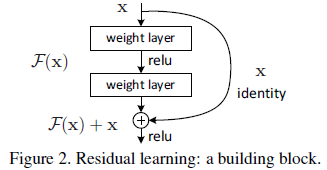
\includegraphics[scale=1]{network_architecture.png}
					\renewcommand{\figurename}{Fig} % set picture title starting with Fig or 图
					\caption{shortcut connection}
					\label{fig3:shortcut connection}
				\end{figure}
		
		\subsection{\quad the two way}
			\begin{itemize}
				\item shortcut 同等维度映射, $F(x)$  与 x 相加就是逐元素相加
					\begin{align}
						y &= F(x, W_i) + x \\
						F &= W_2 \sigma(W_1 x)
					\end{align}
					
				\item 如果两者维度不同, 不要给 x 执行一个线性映射来匹配维度
					\begin{align}
						y &= F(x, W_i) + W_s x\\
						F &= W_2 \sigma(W_1 x)
					\end{align}
			\end{itemize}
			用卷积层进行残差学习: 以上公式表示为了简化, 都是基于全连接层的, 实际上当然可以用于卷积层. 加法随之变为对应 channel 间的两个 feature map 逐元素相加.
			
		\subsection{\quad rule with design network}
			\begin{enumerate}
				\item 对于输出 feature map 大小相同的层, 有相同数量的 filters, 即 channel 数相同
				
				\item 当 feature map 大小减半时 (池化), filters 数量翻倍
					
						\textcolor{red}{对于残差网络, 维度匹配的 shortcut 连接为实线, 反之为虚线.}
						
						维度不同时, 同等映射有两种可选方案:
							\begin{itemize}
								\item 直接通过 zero padding 来增加维度 (channel), 参数 free
								
								\item 乘以 W 矩阵投影到新的空间, 实现是用 $1\times 1$ 卷积实现的, 直接改变 $1 \times 1$ 卷积的 filters 数目, 这种会增加参数
							\end{itemize}
						作者比较了两种方法的优劣, 实验证明, 投影法会比 zero padding 表现稍好一些. 因为 zero padding 的部分没有参与残差学习. 
						
						实验证明, 将维度不同或不匹配的同等映射全用投影法会取得更稍好的结果, 但是考虑到不增加复杂度和参数 free, 不采用这种方法	
					
				\item 图 \ref{fig3:shortcut connection} 是文章里的图, 我们可以看到一个 “弯弯的弧线”, 这个就是所谓的 “shortcut connection”, 也是文中提到 identity mapping, 这张图也诠释了 ResNet 的真谛, 当然大家可以放心, 真正在使用的 ResNet 模块并不是这么单一, 文章中就提出了两种方式:
					\begin{figure}[H]
						\vspace{-0.3cm}  %调整图片与上文的垂直距离
						\setlength{\abovecaptionskip}{-0.05cm}   %调整图片标题与图距离
						%\setlength{\belowcaptionskip}{-1cm}   %调整图片标题与下文距离
						\centering
						\subfigure[bulid block]{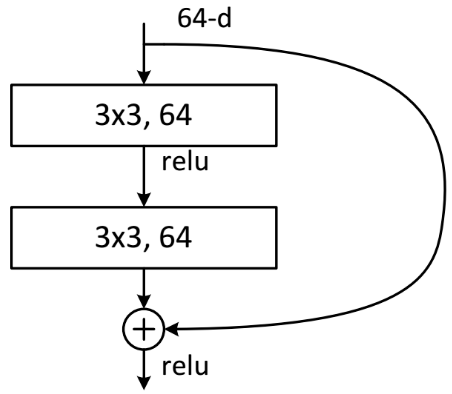
\includegraphics[height=5cm,width=6cm]{build_block1.png}}
						%scale=0.6, height=4cm,width=4cm
						\qquad
						\subfigure[bottleneck design]{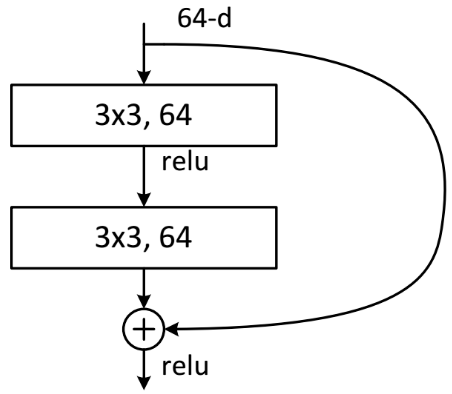
\includegraphics[height=5cm,width=6cm]{build_block1.png}}
						\renewcommand{\figurename}{Fig} % set picture title starting with Fig or 图
						\caption{two design of ResNet}
						\label{fig4:build block}
					\end{figure}
				这两种结构分别针对 ResNet34 (左图) 和 ResNet 50/101/152 (右图), 一般称整个结构为一个 "building block". 
				
				其中右图又称为 "bottleneck design", 目的一目了然, 就是为了降低参数的数目, \textcolor{red}{第一个 $1\times 1$ 的卷积把 256 维 channel 降到 64 维, 然后在最后通过 $1 \times 1$ 卷积恢复}, 整体上用的参数数目为:
					$$1 \times 1 \times 256 \times 64 + 3\times 3\times 64 \times 64 + 1 \times 1 \times 64\times 256 = 69632$$
				而不使用 bottleneck 的话就是两个 $3 \times 3 \times 256$ 的卷积, 参数数目:
					$$3 \times 3 \times 256 \times 256 \times 2 = 1179648$$
				, 差了 16.94 倍.
				
				对于常规 ResNet, 可以用于 34 层或者更少的网络中, 对于 Bottleneck Design 的 ResNet 通常用于更深的如 101 这样的网络中, 目的是减少计算和参数量 (实用目的)
			\end{enumerate}
			
	\section{\quad detail problem}
		\subsection{\quad channel question1}
			如图 \ref{fig3:shortcut connection} 所示, 如果 $F(x)$ 和 x 的 channel 个数不同怎么办, 因为 $F(x)$ 和 x 是按照 channel维度相加的, channel 不同怎么相加呢?
			
			\quad 针对 channel 个数是否相同, 要分成两种情况考虑, 如下图:
				\begin{figure}[H]
					\vspace{-0.2cm}  %调整图片与上文的垂直距离
					\setlength{\abovecaptionskip}{-0.2cm}   %调整图片标题与图距离
					%\setlength{\belowcaptionskip}{-1cm}   %调整图片标题与下文距离
					\centering
					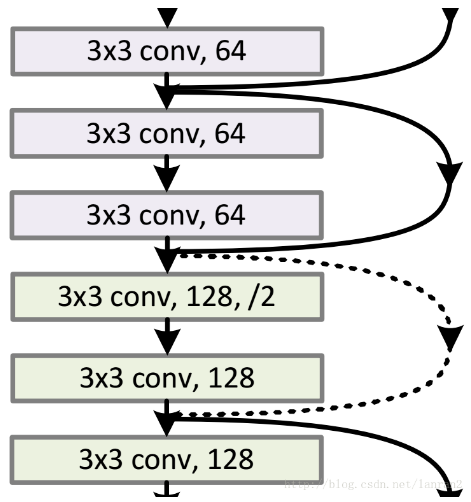
\includegraphics[scale=0.6]{shortcut_connection.png}
					\renewcommand{\figurename}{Fig} % set picture title starting with Fig or 图
					\caption{two way of shortcut connection}
					\label{fig5:shortcut_connection}
				\end{figure}
			如图 \ref{fig5:shortcut_connection} 所示, 我们可以清楚的看到 "实线" 和 "虚线" 两种连接方式, 实线的 Connection 部分 ("第一个粉红色矩形和第三个粉红色矩形") 都是执行 $3\times 3 \times 64$ 的卷积, 它们的 channel 个数一致, 所以采用计算方式:
				\begin{align}
					y = F(x) + x
				\end{align}
			\qquad 虚线的 Connection 部分 ("第一个绿色矩形和第三个绿色矩形") 分别是 $3\times 3 \times 64$ 和 $3\times 3 \times 128$ 的卷积操作, 它们的 channel 个数不同 (64 和 128), 所以采用计算方式:
				\begin{align}
					y = F(x) = Wx
				\end{align}
			其中, W 是卷积操作 (用128个 $(3\times 3)\times 64$ 的 filter), 用来调整 x 的channel 维度的
			
		\subsection{\quad calculate detail}
			\begin{itemize}
				\item 这里的 residual block 和上面 building block 是一个东西
						\begin{figure}[H]
							\vspace{-0.2cm}  %调整图片与上文的垂直距离
							\setlength{\abovecaptionskip}{-0.2cm}   %调整图片标题与图距离
							%\setlength{\belowcaptionskip}{-1cm}   %调整图片标题与下文距离
							\centering
							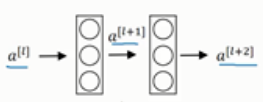
\includegraphics[scale=1.5]{residual_block.png}
							\renewcommand{\figurename}{Fig} % set picture title starting with Fig or 图
							\caption{forward propagation}
							\label{fig6:forward ropagation}
						\end{figure}
						这是一个两层神经网络,在 l 层进行激活,得到$a[l+1]$,再次进行激活, 两层之后得到$a[l+2]$. 计算过程是从$a[l]$开始, 首先进行线性激活, 根据这个公式:$z=wx+b$,通过算出z,即 x (图中$a[l]$) 乘以权重矩阵 w,再加上偏差因子b. 然后通过 ReLU 非线性激活函数得到 a, 计算得出$a[l+1]$. 接着再次进行线性激活, 依据等式$z = wx+b$, 最后根据这个等式再次进行 ReLu 非线性激活, 即, 这里的是指 ReLU 非线性函数, 得到的结果就是$a[l+2]$. 换句话说, 信息流从输入到输出需要经过以上所有步骤, 即这组网络层的主路径. 
						
				\item 在残差网络中做了一些改变, 我们将 输入 直接向后, 拷贝到神经网络的深层, 在 ReLU 非线性激活函数前加上, 这是一条捷径. $a[l]$ 的信息直接到达神经网络的深层, 不再沿着主路径传递, 这就意味着最后这个等式$(a[l+1]=g(wa[l]+b))$去掉了,取而代之的是另一个ReLU非线性函数, 仍然对 $a[l+1]$进行g函数处理, 但这次要加上$a[l]$, 即:$a[l+2]=g(wa[l+1]+b+a[l])$, 也就是加上的这个产生了一个残差块. 
						\begin{figure}[H]
							\vspace{-0.2cm}  %调整图片与上文的垂直距离
							\setlength{\abovecaptionskip}{-0.2cm}   %调整图片标题与图距离
							%\setlength{\belowcaptionskip}{-1cm}   %调整图片标题与下文距离
							\centering
							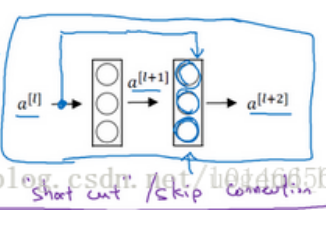
\includegraphics[scale=1]{residual_block_shortcut_connection.png}
							\renewcommand{\figurename}{Fig} % set picture title starting with Fig or 图
							\caption{residual block shortcut connection}
							\label{fig7:residual block shortcut connection}
						\end{figure}
			
				\item 在上面这个图中,我们也可以画一条捷径,直达第二层。实际上这条捷径是在进行ReLU非线性激活函数之前加上的,而这里的每一个节点都执行了线性函数和ReLU激活函数。所以插入的时机是在线性激活之后,ReLU激活之前。除了捷径,你还会听到另一个术语“跳跃连接”,就是指跳过一层或者好几层,从而将信息传递到神经网络的更深层。
				
				\item 这里用的是全连接层举例的, 但是如果在 CNN 中, 如果 \textcolor{red}{残差块 仅是一层 就变成了线性函数}, 实验结果没有多少效果, 所以一般选用的是两层或多层
			\end{itemize}
			
		\subsection{\quad 网络中的网络 及 $1 \times 1$ convolution}
			通常称为 $1×1$ 卷积,有时也被称为Network in Network
			\begin{enumerate}
				\item question: 在架构内容设计方面,其中一个比较有帮助的想法是使用 $1 \times 1$ 卷积。也许你会好奇,1×1的卷积能做什么呢?不就是乘以数字么?听上去挺好笑的,结果并非如此,我们来具体看看
				
				\item 当对于 $6 \times 6 \times 1$ 的一个通道图片来说卷积效果不大
						\begin{figure}[H]
							\vspace{-0.2cm}  %调整图片与上文的垂直距离
							\setlength{\abovecaptionskip}{-0.2cm}   %调整图片标题与图距离
							%\setlength{\belowcaptionskip}{-1cm}   %调整图片标题与下文距离
							\centering
							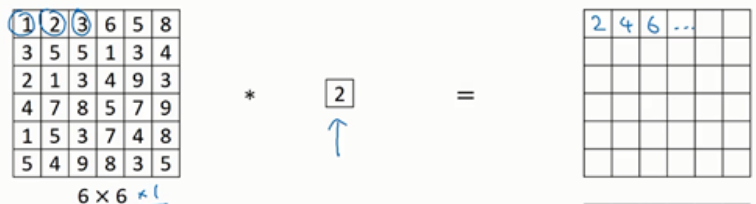
\includegraphics[scale=0.6]{for_6_6_1.png}
							\renewcommand{\figurename}{Fig} % set picture title starting with Fig or 图
							\caption{1 $\times$ 1 convolution for 6 $\times$ 6 $\times$ 1}
							\label{fig8: for 6 6 1}
						\end{figure}
						过滤器为 $1\times 1$, 这里是数字2, 输入一张 $6 \times 6 \times 1$ 的图片, 然后对它做卷积, 起过滤器大小为 $1 \times 1 \times 1$, 结果相当于把这个图片乘以数字2, 所以前三个单元格分别是2、4、6等等。用 $1 \times 1$ 的过滤器进行卷积, 似乎用处不大 ,只是对输入矩阵乘以某个数字
								
				\item 如果是一张 $6\times 6\times 32$ 的图片,那么使用 $1\times 1$ 过滤器进行卷积效果更好
						\begin{figure}[H]
							\vspace{-0.2cm}  %调整图片与上文的垂直距离
							\setlength{\abovecaptionskip}{-0.2cm}   %调整图片标题与图距离
							%\setlength{\belowcaptionskip}{-1cm}   %调整图片标题与下文距离
							\centering
							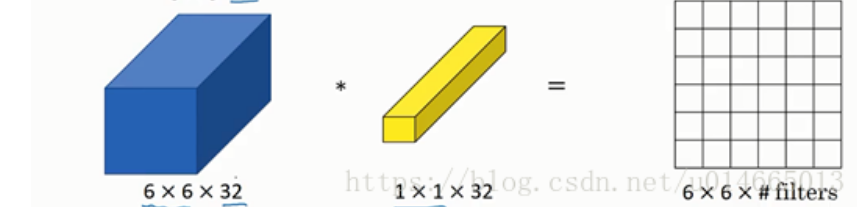
\includegraphics[scale=0.6]{for_6_6_32.png}
							\renewcommand{\figurename}{Fig} % set picture title starting with Fig or 图
							\caption{1 $\times$ 1 convolution for 32 $\times$ 6 $\times$ 1}
							\label{fig9: for 6 6 32}
						\end{figure}
					具体来说,$1 \times 1$ 卷积所实现的功能是遍历这36个单元格,计算左图中32个数字和过滤器中32个数字的元素积之和,然后应用ReLU非线性函数。
					
				\item 以其中一个单元为例,它是这个输入层上的某个切片,用这36个数字乘以这个输入层上 $1 \times 1$ 切片,得到一个实数,像这样把它画在输出中
						\begin{figure}[H]
							\vspace{-0.2cm}  %调整图片与上文的垂直距离
							\setlength{\abovecaptionskip}{-0.2cm}   %调整图片标题与图距离
							%\setlength{\belowcaptionskip}{-1cm}   %调整图片标题与下文距离
							\centering
							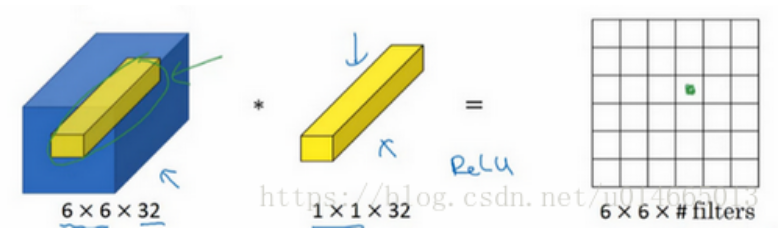
\includegraphics[scale=0.6]{2_for_6_6_32.png}
							\renewcommand{\figurename}{Fig} % set picture title starting with Fig or 图
							\caption{one unit of 1 $\times$ 1 convolution for 32 $\times$ 6 $\times$ 1}
							\label{fig10: one unit for 6 6 32}
						\end{figure}
					
				\item 这个 $1 \times 1 \times 32$ 过滤器中的32个数字可以这样理解,一个神经元的输入是32个数字(输入图片中左下角位置32个通道中的数字), 即相同高度和宽度上某一切片上的32个数字, 这32个数字具有不同通道, 乘以32个权重 (将过滤器中的32个数理解为权重),  然后应用 ReLU 非线性函数, 在这里输出相应的结果.
						\begin{figure}[H]
							\vspace{-0.2cm}  %调整图片与上文的垂直距离
							\setlength{\abovecaptionskip}{-0.2cm}   %调整图片标题与图距离
							%\setlength{\belowcaptionskip}{-1cm}   %调整图片标题与下文距离
							\centering
							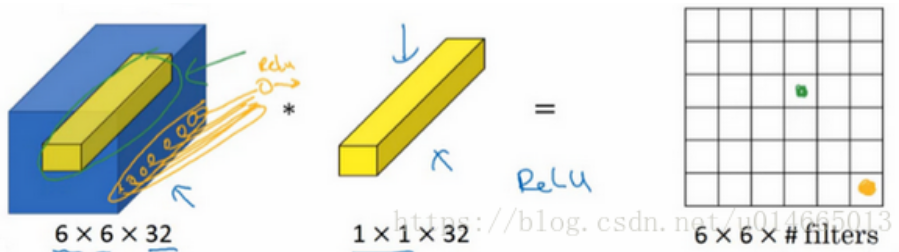
\includegraphics[scale=0.5]{3_for_6_6_32.png}
							\renewcommand{\figurename}{Fig} % set picture title starting with Fig or 图
							\caption{one2 unit of 1 $\times$ 1 convolution for 32 $\times$ 6 $\times$ 1}
							\label{fig11: one unit for 6 6 32}
						\end{figure}
					
				 \item 一般来说, 如果过滤器不止一个, 而是多个, 就好像有多个输入单元, 其输入内容为一个切片上所有数字, 输出结果是 $6×6$ 过滤器数量
				 			\begin{figure}[H]
				 				\vspace{-0.2cm}  %调整图片与上文的垂直距离
				 				\setlength{\abovecaptionskip}{-0.2cm}   %调整图片标题与图距离
				 				%\setlength{\belowcaptionskip}{-1cm}   %调整图片标题与下文距离
				 				\centering
				 				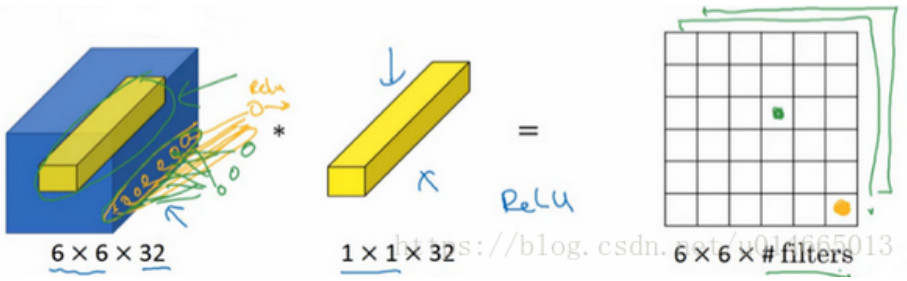
\includegraphics[scale=0.5]{4_for_6_6_32.png}
				 				\renewcommand{\figurename}{Fig} % set picture title starting with Fig or 图
				 				\caption{one3 unit of 1 $\times$ 1 convolution for 32 $\times$ 6 $\times$ 1}
				 				\label{fig12: one unit for 6 6 32}
				 			\end{figure}
			 
			 	\item 所以 $1 \times 1$ 卷积可以从根本上理解为对这 32 个不同的位置都应用一个全连接层, 全连接层的作用是输入32个数字 (过滤器数量标记为, 在这36个单元上重复此过程), 输出结果是 $6 \times 6 \times \#$ filters (锅炉器数量), 以便在输入层上实施一个非平凡 (non-trivial) 计算
			 				\begin{figure}[H]
			 					\vspace{-0.2cm}  %调整图片与上文的垂直距离
			 					\setlength{\abovecaptionskip}{-0.2cm}   %调整图片标题与图距离
			 					%\setlength{\belowcaptionskip}{-1cm}   %调整图片标题与下文距离
			 					\centering
			 					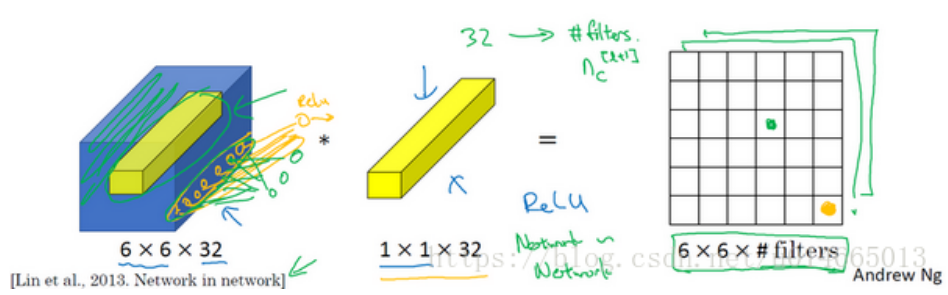
\includegraphics[scale=0.5]{5_for_6_6_32.png}
			 					\renewcommand{\figurename}{Fig} % set picture title starting with Fig or 图
			 					\caption{one4 unit of 1 $\times$ 1 convolution for 32 $\times$ 6 $\times$ 1}
			 					\label{fig13: one unit for 6 6 32}
			 				\end{figure}
			 	
			 	\item example
			 	
			 		假设这是一个 $28 \times 28 \times 192$ 的输入层, 你可以使用池化层压缩它的高度和宽度, 这个过程我们很清楚. 但如果通道数量很大, 该如何把它压缩为 $28 \times 28 \times 32$ 维度的层呢? 你可以用32个大小为 $1 \times 1$ 的过滤器, 严格来讲每个过滤器大小都是 $1 \times 1 \times 192$ 维, 因为过滤器中通道数量必须与输入层中通道的数量保持一致.  但是你使用了32个过滤器, 输出层为 $28 \times 28 \times 32$, 这就是压缩通道数 () 的方法, 对于池化层我只是压缩了这些层的高度和宽度
						\begin{figure}[H]
							\vspace{-0.2cm}  %调整图片与上文的垂直距离
							\setlength{\abovecaptionskip}{-0.2cm}   %调整图片标题与图距离
							%\setlength{\belowcaptionskip}{-1cm}   %调整图片标题与下文距离
							\centering
							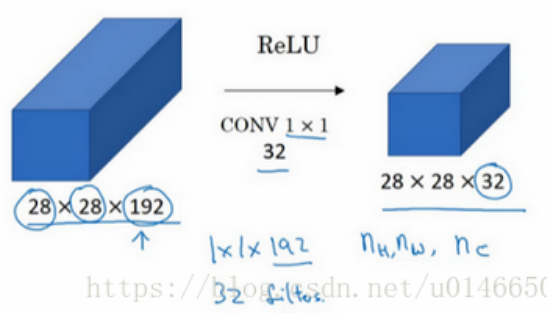
\includegraphics[scale=0.5]{example_network_in_network.png}
							\renewcommand{\figurename}{Fig} % set picture title starting with Fig or 图
							\caption{example of 1 $\times$ 1 convolution}
							\label{fig14: example network in network}
						\end{figure}
					
				\item 在之后我们看到在某些网络中1×1卷积是如何压缩通道数量并减少计算的. 当然如果你想保持通道数192不变, 这也是可行的, $1 \times 1$ 卷积只是添加了非线性函数, 当然也可以让网络学习更复杂的函数, 比如, 我们再添加一层, 其输入为 $28\times 28\times 192$, 输出为 $28\times 28\times 192$.
						\begin{figure}[H]
							\vspace{-0.2cm}  %调整图片与上文的垂直距离
							\setlength{\abovecaptionskip}{-0.2cm}   %调整图片标题与图距离
							%\setlength{\belowcaptionskip}{-1cm}   %调整图片标题与下文距离
							\centering
							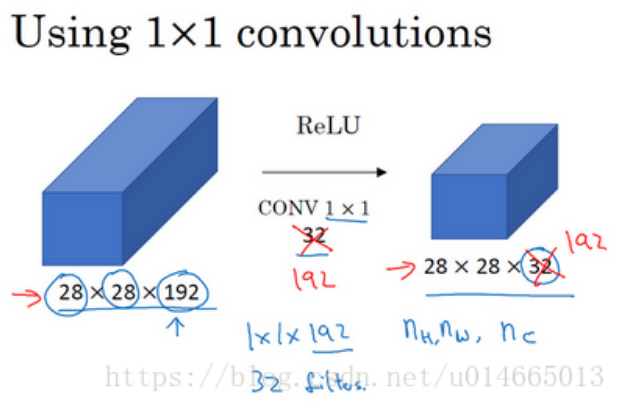
\includegraphics[scale=0.5]{example2_network_in_network.png}
							\renewcommand{\figurename}{Fig} % set picture title starting with Fig or 图
							\caption{example2 of 1 $\times$ 1 convolution}
							\label{fig15: example2 network in network}
						\end{figure}
					
				\item $1\times 1$ 卷积层就是这样实现了一些重要功能的 (doing something pretty non-trivial), 它给神经网络添加了一个非线性函数, 从而减少或保持输入层中的通道数量不变, 当然如果你愿意, 也可以增加通道数量.
			\end{enumerate}

	\section{\quad ResNet50 and ResNet101}
		这里把ResNet50和ResNet101特别提出,主要因为它们的出镜率很高
			\begin{figure}[H]
				\vspace{-0.2cm}  %调整图片与上文的垂直距离
				\setlength{\abovecaptionskip}{-0.2cm}   %调整图片标题与图距离
				%\setlength{\belowcaptionskip}{-1cm}   %调整图片标题与下文距离
				\centering
				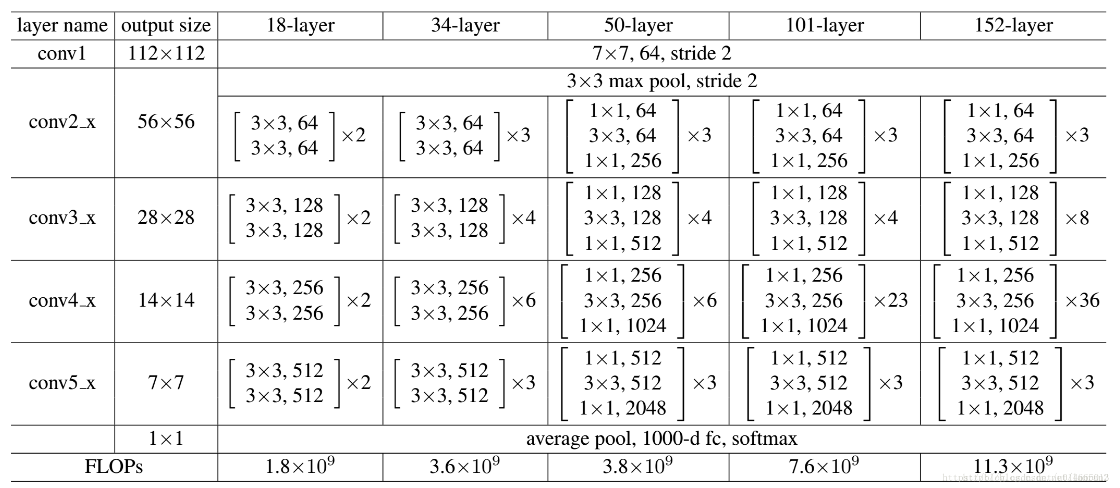
\includegraphics[scale=0.5]{ResNet50_and_ResNet101.png}
				\renewcommand{\figurename}{Fig} % set picture title starting with Fig or 图
				\caption{ResNet50 and ResNet101}
				\label{fig16:ResNet50 and ResNet101 }
			\end{figure}
		\begin{itemize}
			\item 首先我们看一下表2,上面一共提出了5中深度的ResNet, 分别是18,34,50,101和152, 首先看图 \ref{fig16:ResNet50 and ResNet101 } 最左侧,我们发现所有的网络都分成 5 部分,分别是:$conv1,conv2\_x,conv3\_x,conv4\_x,conv5\_x,$之后的其他论文也会专门用这个称呼指代ResNet50或者101的每部分.。
	
			\item 拿101-layer那列, 我们先看看101-layer是不是真的是101层网络, 首先有个输入 $7\times 7\times 64$的卷积, 然后经过 $3 + 4 + 23 + 3 = 33$ 个building block, 每个block为3层, 所以有 $33 \times 3 = 99$ 层, 最后有个fc层(用于分类), 所以 $1 + 99 + 1 = 101$ 层, 确实有101层网络

			\item 注:101层网络仅仅指卷积或者全连接层, 而激活层或者Pooling层并没有计算在内
			
			\item 这里我们关注50-layer和101-layer这两列, 可以发现, 它们唯一的不同在于$conv4\_x, ResNet50$有6个block, 而ResNet101有23个block, 查了17个block, 也就是 $17 \times 3 = 51$ 层
		\end{itemize}
	
	\section{\quad related work}
		\subsection{\quad 残差表示}
			VALD,Fisher Vector都是是对残差向量编码来表示图像,在图像分类,检索表现出优于编码原始向量的性能.\\
			在low-level的视觉和计算机图形学中,为了求解偏微分方程,广泛使用的Multigrid方法将系统看成是不同尺度上的子问题.每个子问题负责一种更粗糙与更精细尺度的残差分辨率.Multigrid的一种替换方法是层次化的预处理,层次化的预处理依赖于两种尺度的残差向量表示.实验表明,这些求解器要比对残差不敏感的求解器收敛更快

		\subsection{\quad shortcut connection}
			普通的平原网络与深度残差网络的最大区别在于,深度残差网络有很多旁路的支线将输入直接连到后面的层,使得后面的层可以直接学习残差,这些支路就叫做shortcut。传统的卷积层或全连接层在信息传递时,或多或少会存在信息丢失、损耗等问题.ResNet 在某种程度上解决了这个问题,通过直接将输入信息绕道传到输出,保护信息的完整性,整个网络则只需要学习输入、输出差别的那一部分,简化学习目标和难度.
			\begin{figure}[H]
				\vspace{-0.2cm}  %调整图片与上文的垂直距离
				\setlength{\abovecaptionskip}{-0.2cm}   %调整图片标题与图距离
				%\setlength{\belowcaptionskip}{-1cm}   %调整图片标题与下文距离
				\centering
				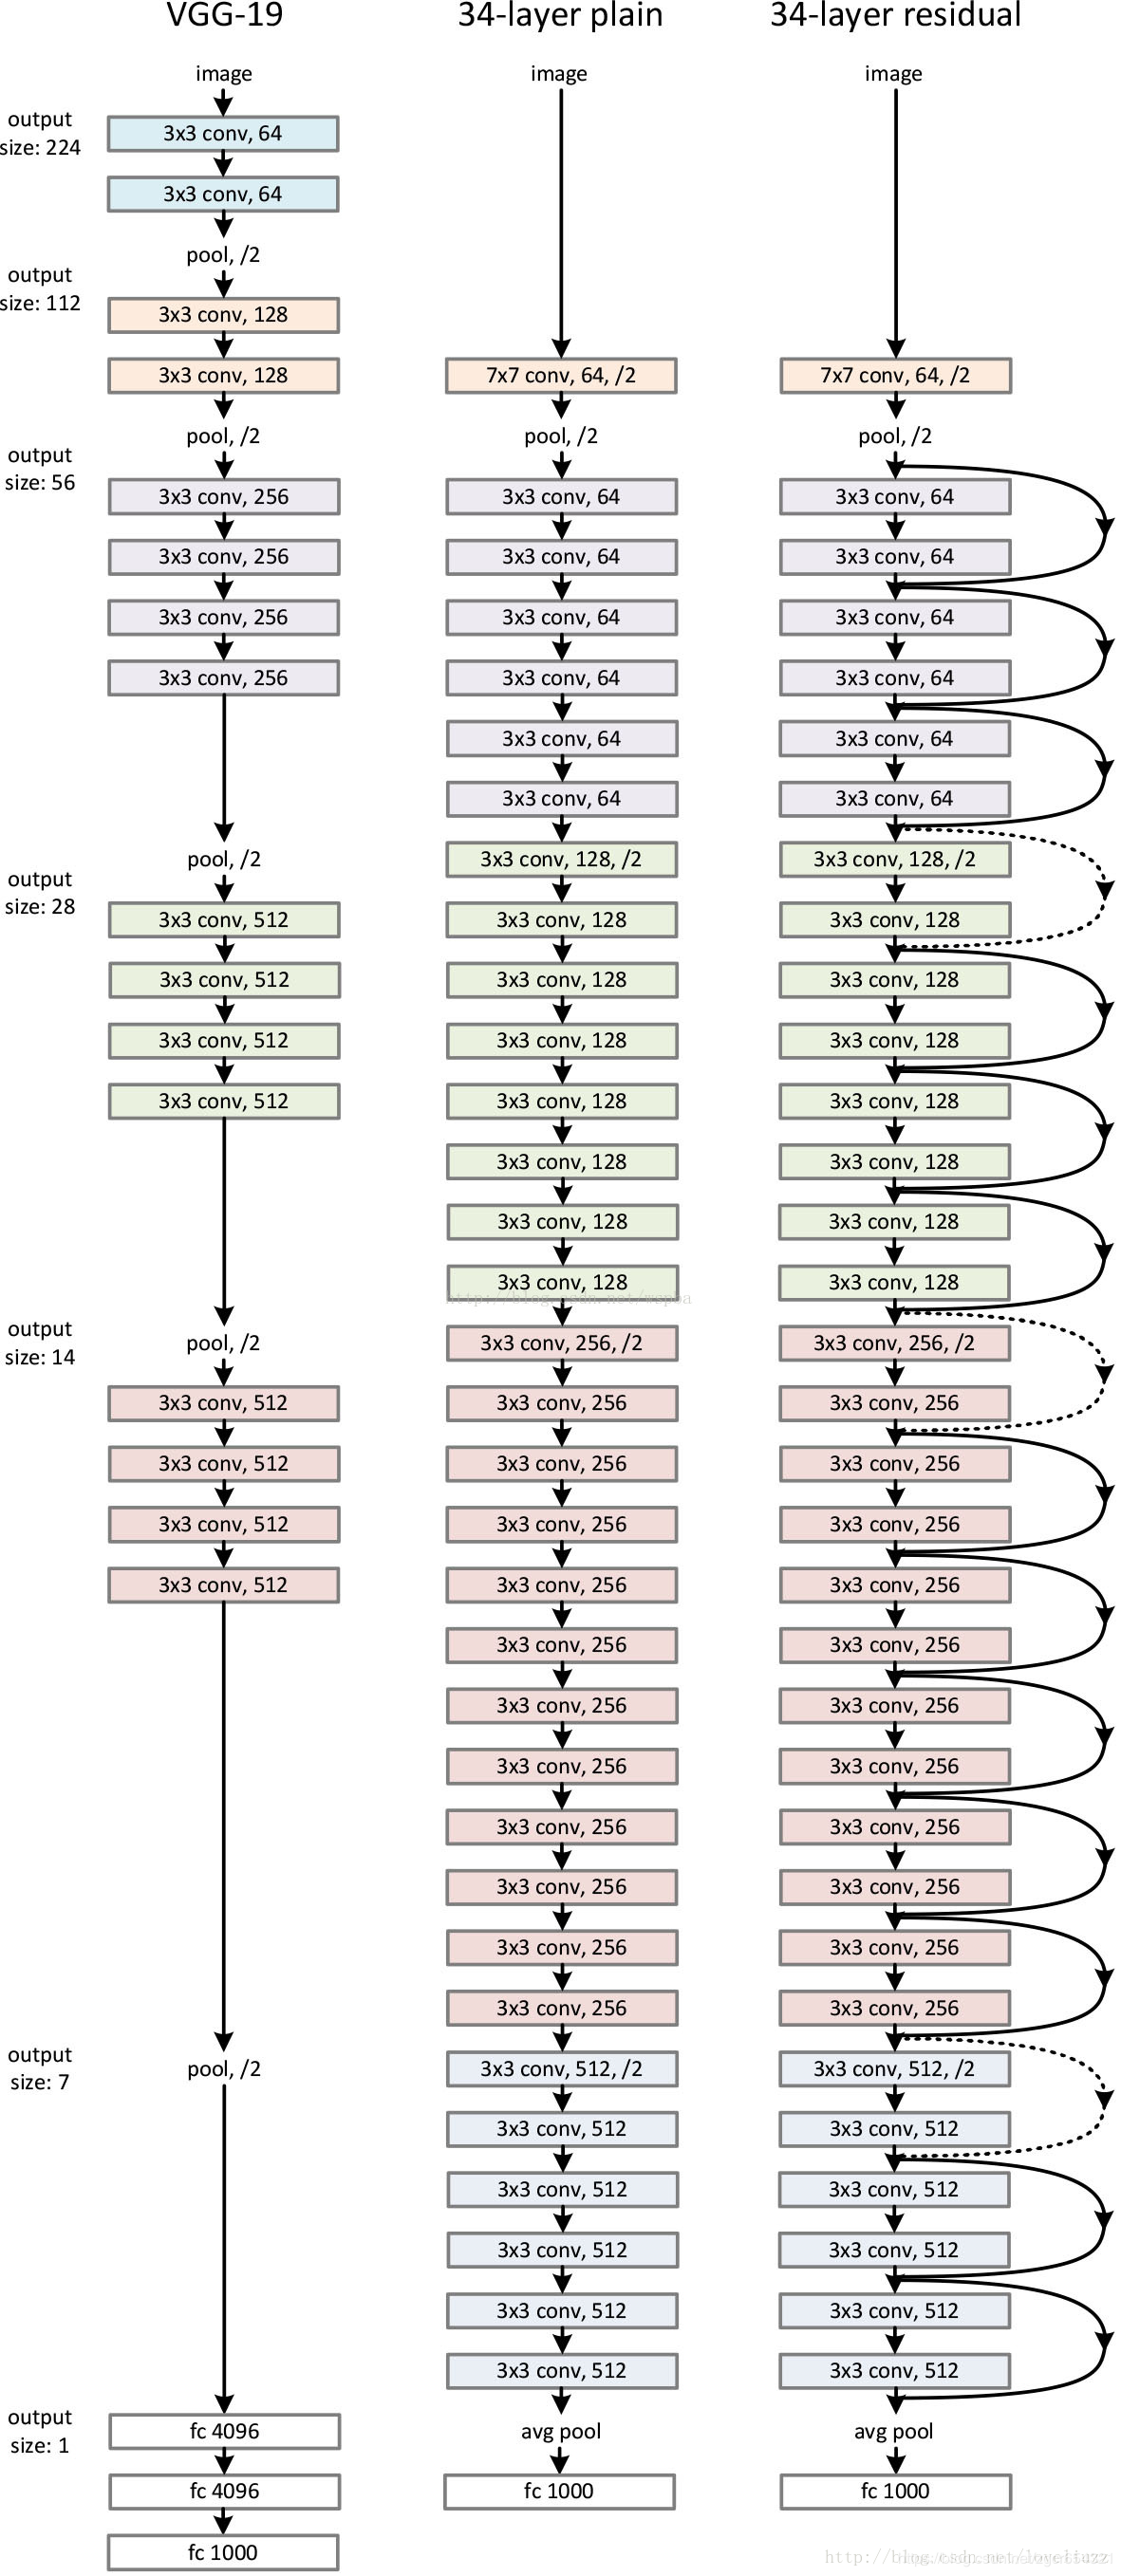
\includegraphics[height=20cm,width=12cm]{vgg_plain_residual.png}
				\renewcommand{\figurename}{Fig} % set picture title starting with Fig or 图
				\caption{vgg plain residual}
				\label{fig17:vgg plain residual}
			\end{figure}
		
	\section{\quad new residual network}
		在残差网络提出之后的一年,有人对其做了大量的研究并提出了一种经过优化后的残差网络,如下图 \ref{fig18:new_residual_net} (b)所示:
			\begin{figure}[H]
				\vspace{-0.2cm}  %调整图片与上文的垂直距离
				\setlength{\abovecaptionskip}{-0.2cm}   %调整图片标题与图距离
				%\setlength{\belowcaptionskip}{-1cm}   %调整图片标题与下文距离
				\centering
				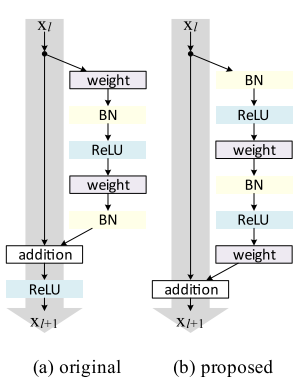
\includegraphics[scale=0.8]{new_residual_net.png}
				\renewcommand{\figurename}{Fig} % set picture title starting with Fig or 图
				\caption{new residual net}
				\label{fig18:new_residual_net}
			\end{figure}
		这个其实就是作者通过大量的试验,去调整了Batch Normalization和激活函数的位置,最后提出的不要对先前addition之后的结果再激活了,而是放到神经网络层之间去处理。很多先进的框架都使用了这种结构,比如在QANet中。公式就变成了:
			\begin{align}
				x_{l+1} = x_l + F(x_l, w_l)
			\end{align}
			
	\section{\quad other knowleadge}
		\begin{itemize}	
			\item 请问博主,既然最终拟合的是一个恒等映射 $h(x)=x$,那还干嘛要去拟合,直接用x不就行了吗? 或者说既然优化的目的是使得F(X)尽可能趋于0,那么一开始不要这部分不行吗? 虽然我知道不要这部分网络就变浅了,但要了这部分又来将它优化为0,岂不矛盾了吗
				\begin{enumerate}
					\item 除了文章本身说的,有人从模型ensemble角度揭示了resnet的本质 (它并不深,绕开了极深网络的训练问题,而不是解决了这个问题), 说Residual不是必须的, 影响网络ensemble个数的是深度和单block分支数. 因此,densenet就出来了,它使得任意两层之间建立前向skip connetion
					
					\item 就算是拟合残差,也只能保证冗余的网络层变成恒等映射,使得更深网络的性能不会降低。那resnet是如何做到提升的呢?
					
					\item 拟合残差咯
				\end{enumerate}
				
			\item 楼主,我最近也看了Deep Residual Learning for Image Recognition这篇文章,想问一下上图网络结构中,可以理解为实线部分是恒等映射,而虚线部分则需要学习残差吗? 
			
			虚线是说发生了输出的增维,即比如输出的channel个数从64变成了128。相对实线,它多了一个1x1的卷积来将channel个数从64增加到128个
			
			\item 计算机视觉里,特征的“等级”随增网络深度的加深而变高,研究表明,网络的深度是实现好的效果的重要因素。然而梯度弥散/爆炸成为训练深层次的网络的障碍,导致无法收敛。
			
			有一些方法可以弥补,如归一初始化,各层输入归一化,使得可以收敛的网络的深度提升为原来的十倍。然而,虽然收敛了,但网络却开始退化了,即增加网络层数却导致更大的误差, 如下图。 这种deep plain net收敛率十分低下。
				\begin{figure}[H]
					\vspace{-0.2cm}  %调整图片与上文的垂直距离
					\setlength{\abovecaptionskip}{-0.2cm}   %调整图片标题与图距离
					%\setlength{\belowcaptionskip}{-1cm}   %调整图片标题与下文距离
					\centering
					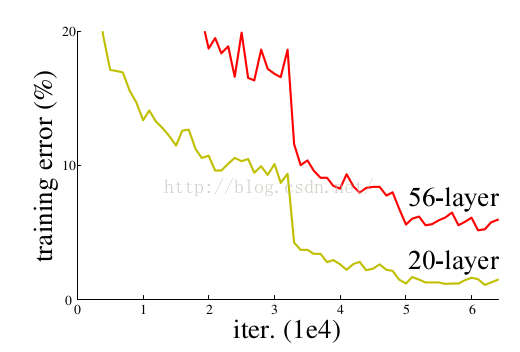
\includegraphics[scale=0.5]{converge_way.png}
					\renewcommand{\figurename}{Fig} % set picture title starting with Fig or 图
					\caption{converge way}
					\label{fig19:converge way}
				\end{figure}
			的确,通过在一个浅层网络基础上叠加y=x的层(称identity mappings,恒等映射),可以让网络随深度增加而不退化。这反映了多层非线性网络无法逼近恒等映射网络。
			
			\item  resnet学习的是残差函数$F(x) = H(x) - x$, 这里如果$F(x) = 0$, 那么就是上面提到的恒等映射。事实上,resnet是 “shortcut connections” 的在 connections 是在恒等映射下的特殊情况,它没有引入额外的参数和计算复杂度。 假如优化目标函数是逼近一个恒等映射, 而不是0映射, 那么学习找到对恒等映射的扰动会比重新学习一个映射函数要容易。从下图可以看出,残差函数一般会有较小的响应波动,表明恒等映射是一个合理的预处理。
				\begin{figure}[H]
					\vspace{-0.2cm}  %调整图片与上文的垂直距离
					\setlength{\abovecaptionskip}{-0.2cm}   %调整图片标题与图距离
					%\setlength{\belowcaptionskip}{-1cm}   %调整图片标题与下文距离
					\centering
					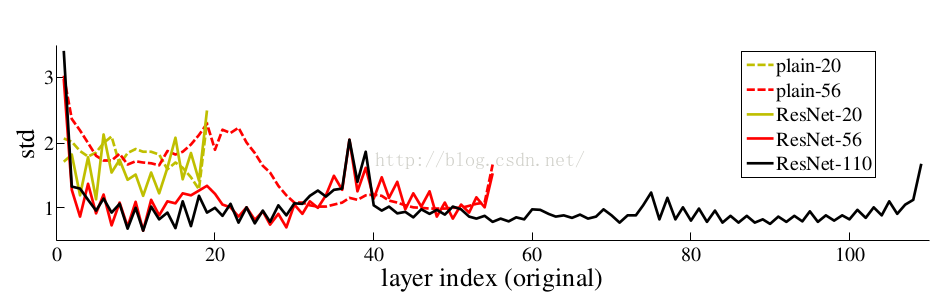
\includegraphics[height=6cm,width=14cm]{net.png}
					\renewcommand{\figurename}{Fig} % set picture title starting with Fig or 图
					\caption{identity mapping}
					\label{fig20:net}
				\end{figure}
		\end{itemize}
\end{document}}